\documentclass[10pt,a4paper]{article}

\usepackage[T1]{fontenc}
\usepackage[utf8]{inputenc}
\usepackage[english]{babel}
\usepackage{geometry}
\geometry{top=2.2cm,bottom=2.3cm,left=2.2cm,right=2.2cm}

\usepackage{amsmath,amssymb,bm}
\setcounter{MaxMatrixCols}{20}
\usepackage{graphicx}
\usepackage{xcolor}
\usepackage{tcolorbox}
\tcbuselibrary{skins,breakable}
\usepackage{booktabs}
\usepackage{fancyhdr}
\usepackage{caption}
\usepackage{float}
\usepackage{listings}
\usepackage{tikz}
\usetikzlibrary{arrows.meta,positioning,calc}
\usepackage[hidelinks]{hyperref}

% ---------------------------------------------------------- metadata ---
\newcommand{\Institution}{Instituto Superior Técnico}
\newcommand{\Programme}{MEAer}
\newcommand{\CourseTitle}{Unmanned Aerial Vehicles}
\newcommand{\ReportTitle}{Estimation of Motion Variables of the Parrot AR.Drone}
\newcommand{\LabNumber}{2}
\newcommand{\Semester}{2026/2027 -- First Semester}
\newcommand{\GroupNumber}{17}            % TODO: group number
\newcommand{\Instructor}{Prof.\ David Cabecinhas}

% name / number / (one line per author)
\newcommand{\AuthorList}{%
  \AuthorRow{IST1116311}{Caio Hokama Freitas}%
  \AuthorRow{IST1113325}{Majid Atarzadeh}%   TODO: real IST number
}

% ------------------------------------------------------------ colours ---
\definecolor{istblue}{HTML}{03ABE6}
\definecolor{qfill}{HTML}{E4F6FD}
\definecolor{qtitle}{HTML}{0288B0}
\definecolor{greyfill}{HTML}{F7F7F7}
\definecolor{greyline}{HTML}{D9D9D9}
\definecolor{tagT}{HTML}{B45309}
\definecolor{tagL}{HTML}{2E7D32}

% ------------------------------------------------- header and footer ---
\pagestyle{fancy}
\fancyhf{}
\fancyhead[L]{\footnotesize IST}
\fancyhead[R]{\footnotesize ULisboa}
\fancyfoot[C]{\footnotesize\thepage}
\renewcommand{\headrulewidth}{0.6pt}
\renewcommand{\footrulewidth}{0.4pt}

% ------------------------------------------- question / answer boxes ---
% #1 is T or L; the colours are named tagT and tagL.
\newcommand{\tagpill}[1]{%
  \begingroup
  \setlength{\fboxsep}{2pt}%
  \colorbox{tag#1}{\textcolor{white}{\scriptsize\bfseries~#1~}}%
  \endgroup}

% \tagpills{T}, \tagpills{L}, \tagpills{T+L} or \tagpills{T + L}: one pill per tag, joined by "+".
\makeatletter
\newcommand{\tagpills}[1]{%
  \edef\tagpills@list{\zap@space#1 \@empty}%
  \expandafter\tagpills@next\tagpills@list+\@nil}
\def\tagpills@next#1+#2\@nil{%
  \tagpill{#1}%
  \ifx\relax#2\relax\else
    \hspace{3pt}{\small\bfseries\textcolor{qtitle}{+}}\hspace{3pt}%
    \tagpills@next#2\@nil
  \fi}
\makeatother

% \begin{question}{2.1}{T}  ... \end{question}
\newenvironment{question}[2]{%
  \begin{tcolorbox}[breakable,enhanced,colback=qfill,colframe=qfill,
    borderline west={3pt}{0pt}{istblue},boxrule=0pt,arc=2pt,
    left=8pt,right=8pt,top=7pt,bottom=7pt,before skip=12pt,after skip=6pt]
  \textcolor{qtitle}{\bfseries Question #1}\hspace{4pt}\tagpills{#2}\par\vspace{3pt}%
}{\end{tcolorbox}}

\newenvironment{answer}{%
  \begin{tcolorbox}[breakable,enhanced,colback=white,colframe=greyline,
    boxrule=0.6pt,arc=2pt,left=8pt,right=8pt,top=7pt,bottom=7pt,
    before skip=0pt,after skip=12pt]
}{\end{tcolorbox}}

\newcommand{\todoanswer}{\emph{Write your answer here.}}

% ----------------------------------------------------- code listings ---
\lstdefinestyle{mat}{
  language=Matlab, basicstyle=\ttfamily\footnotesize,
  keywordstyle=\color{blue!60!black}, commentstyle=\color{green!40!black},
  stringstyle=\color{purple}, numbers=none, frame=single,
  rulecolor=\color{greyline}, backgroundcolor=\color{greyfill},
  breaklines=true, showstringspaces=false, columns=fullflexible,
}
\lstset{style=mat}

% --------------------------------------------------------- shortcuts ---
\newcommand{\R}{\mathbb{R}}
\newcommand{\fB}{\{B\}}
\newcommand{\fI}{\{I\}}
\newcommand{\Bp}{{}^{B}\bm{p}}

\captionsetup{font=small,labelfont=bf}

% =======================================================================
\begin{document}

% ------------------------------------------------------- cover page ---
\newcommand{\AuthorRow}[2]{%
  \makebox[3.2cm][l]{\textbf{N.\textsuperscript{o}: #1}}%
  \makebox[8.2cm][l]{\textbf{Name: #2}}%
  \textbf{Signature:}\\[1.4ex]}

\begin{titlepage}
\thispagestyle{empty}
\noindent
\includegraphics[width=3.2cm]{figs/ist_logo.png}

\vspace{1.6cm}
\begin{center}
  {\large \Institution}\\[1.0em]
  {\large \Programme}\\[2.4em]
  {\LARGE \bfseries \CourseTitle}\\[1.2em]
  {\normalsize \Semester}

  \vspace{4.2cm}

  {\LARGE \underline{Laboratory \LabNumber}}\\[0.8em]
  {\small \itshape \ReportTitle}\\[1.8em]
  {\normalsize \bfseries \underline{Group \GroupNumber}}
\end{center}

\vspace{1.4em}
\noindent\AuthorList

\vfill
\begin{center}
  {\normalsize \underline{Instructor: \Instructor}}
\end{center}
\vspace{2.2cm}
\end{titlepage}

\setcounter{page}{1}
\setcounter{section}{2}   % the guide's Section 1 (Introduction) is not reproduced

% =====================================================================
\section{Modeling and characterization of the sensors}

% ------------------------------------------------------------ Q3.1 ---
\begin{question}{3.1}{L}
    Characterize the accelerometers and rate gyro disturbances that are present on the measurements, by computing the mean and covariance of the measurements obtained in \emph{Experiment A}.
\end{question}

\begin{answer}
In Experiment A the drone is at rest on the ground with the motors off.
Only the interval $10$--$24$\,s was used ($N=2801$ samples): the first
samples of the log have the accelerometer at zero, and in $0$--$10$\,s and
$25$--$30$\,s the drone was disturbed (the standard deviation of $a_x$ and
$a_y$ doubles and the onboard angles change). The accelerometer is given in mg
and the rate gyro in deg/s. For each sensor, with samples
$\mathbf{x}_k\in\R^3$,
\[
  \boldsymbol{\mu} = \frac{1}{N}\sum_{k=1}^{N}\mathbf{x}_k, \qquad
  \boldsymbol{\Sigma} = \frac{1}{N-1}\sum_{k=1}^{N}
  (\mathbf{x}_k-\boldsymbol{\mu})(\mathbf{x}_k-\boldsymbol{\mu})^T,
\]
and the standard deviations are $\boldsymbol{\sigma}=\sqrt{\mathrm{diag}(\boldsymbol{\Sigma})}$.

\paragraph{Accelerometer}
\[
\boldsymbol{\mu}_{a,A} =
\begin{bmatrix} 12.0\\ -37.8\\ -1011.1 \end{bmatrix}\mathrm{mg},
\qquad
\boldsymbol{\Sigma}_{a,A} =
\begin{bmatrix}
11.59 & -0.57 & -0.28\\
-0.57 & 0.93 & 0.61\\
-0.28 & 0.61 & 10.79
\end{bmatrix}\mathrm{mg}^2,
\qquad
\boldsymbol{\sigma}_{a,A} =
\begin{bmatrix} 3.40\\ 0.96\\ 3.29 \end{bmatrix}\mathrm{mg}.
\]
The norm of the mean is $1011.9$\,mg: at rest the accelerometer
measures only gravity, $-g$ along $z$. The small $x$ and $y$ components
come from the tilt of the ground and from sensor offsets.

\paragraph{Rate gyro}
\[
\boldsymbol{\mu}_{g,A} =
\begin{bmatrix} 0.048\\ -0.085\\ 0.003 \end{bmatrix}\mathrm{deg/s},
\quad
\boldsymbol{\Sigma}_{g,A} =
\begin{bmatrix}
1.76 & 0.02 & -0.09\\
0.02 & 1.77 & 0.10\\
-0.09 & 0.10 & 1.63
\end{bmatrix}\times10^{-3}\,(\mathrm{deg/s})^2,
\quad
\boldsymbol{\sigma}_{g,A} =
\begin{bmatrix} 0.042\\ 0.042\\ 0.040 \end{bmatrix}\mathrm{deg/s}.
\]
The vehicle does not rotate, so the mean is the gyro bias, below
$0.1$\,deg/s in the three axes. In both sensors the covariance is almost
diagonal: the noise of the three axes is uncorrelated. These values are
the intrinsic sensor noise, without disturbances from the motors.
\end{answer}

% ------------------------------------------------------------ Q3.2 ---
\begin{question}{3.2}{L}
    Repeat the previous computations for \emph{Experiment B}. Discuss the new sources of disturbances leading to the increase of uncertainty on the measurements.
\end{question}

\begin{answer}
Same computation as in Q3.1, in the interval $10$--$33$\,s, after the
rotors spin up and the drone settles ($N=4601$); before $10$\,s the drone
is tilted while it is pressed down (onboard roll of about $-3^\circ$).

\paragraph{Accelerometer}
\[
\boldsymbol{\mu}_{a,B} =
\begin{bmatrix} 47.7\\ 61.9\\ -1006.8 \end{bmatrix}\mathrm{mg},
\qquad
\boldsymbol{\Sigma}_{a,B} =
\begin{bmatrix}
297 & 249 & -26\\
249 & 6287 & 289\\
-26 & 289 & 305
\end{bmatrix}\mathrm{mg}^2,
\qquad
\boldsymbol{\sigma}_{a,B} =
\begin{bmatrix} 17.2\\ 79.3\\ 17.5 \end{bmatrix}\mathrm{mg}.
\]

\paragraph{Rate gyro}
\[
\boldsymbol{\mu}_{g,B} =
\begin{bmatrix} -0.14\\ 0.21\\ -0.39 \end{bmatrix}\mathrm{deg/s},
\qquad
\boldsymbol{\Sigma}_{g,B} =
\begin{bmatrix}
27.0 & 6.5 & 21.9\\
6.5 & 10.5 & 11.3\\
21.9 & 11.3 & 34.8
\end{bmatrix}(\mathrm{deg/s})^2,
\qquad
\boldsymbol{\sigma}_{g,B} =
\begin{bmatrix} 5.20\\ 3.24\\ 5.90 \end{bmatrix}\mathrm{deg/s}.
\]

With the rotors on, $\boldsymbol{\sigma}_a$ grows by a factor of about 5
in $x$ and $z$ and 80 in $y$, and $\boldsymbol{\sigma}_g$ by 80 to 150.
The new disturbance is the vibration of the motors and propellers
(unbalance, blade passing), transmitted through the frame to the sensor
board. It is not the same in every direction, and the gyro axes are now
correlated (off-diagonal terms of the order of the variances), as
expected from a mechanical excitation common to the three axes. The mean
of $a_y$ also moves from $-37.8$ to $+61.9$\,mg, so the inclinometer
roll goes from $2.1^\circ$ to $-3.5^\circ$ (Q3.4) with the drone on the
ground. These covariances describe the vibration, not the sensor noise.
\end{answer}

% ------------------------------------------------------------ Q3.3 ---
\begin{question}{3.3}{L}
    Repeat the previous computations for \emph{Experiment C}. Discuss the new sources of disturbances leading to the increase of uncertainty on the measurements.
\end{question}

\begin{answer}
Same computations were performed over the interval \(9\)--\(30\,\mathrm{s}\), corresponding to steady hover. The take-off and landing phases were excluded, resulting in \(N=4201\) samples.

\paragraph{Accelerometer}

\[
\boldsymbol{\mu}_{a,C} =
\begin{bmatrix}
8.0\\ -42.7\\ -1008.6
\end{bmatrix}\mathrm{mg},
\qquad
\boldsymbol{\Sigma}_{a,C} =
\begin{bmatrix}
59.1 & 28.3 & 20.8\\
28.3 & 43.1 & 19.5\\
20.8 & 19.5 & 56.8
\end{bmatrix}\mathrm{mg}^2,
\]
\[
\boldsymbol{\sigma}_{a,C} =
\begin{bmatrix}
7.69\\ 6.57\\ 7.53
\end{bmatrix}\mathrm{mg}.
\]

\paragraph{Rate gyro}

\[
\boldsymbol{\mu}_{g,C} =
\begin{bmatrix}
-0.065\\ 0.040\\ -0.020
\end{bmatrix}\mathrm{deg/s},
\qquad
\boldsymbol{\Sigma}_{g,C} =
\begin{bmatrix}
2.09 & -0.38 & -0.43\\
-0.38 & 2.51 & 0.23\\
-0.43 & 0.23 & 2.55
\end{bmatrix}(\mathrm{deg/s})^2,
\]
\[
\boldsymbol{\sigma}_{g,C} =
\begin{bmatrix}
1.45\\ 1.58\\ 1.60
\end{bmatrix}\mathrm{deg/s}.
\]

Compared with Experiment A, the standard deviations increase by approximately \(2\)--\(7\) times for the accelerometer and \(35\)--\(40\) times for the rate gyro. This increase reflects the disturbances present during flight. Compared with Experiment B, however, the measured standard deviations are considerably lower. In particular, the gyro standard deviations decrease from \(3.24\)--\(5.90\,\mathrm{deg/s}\) in Experiment B to \(1.45\)--\(1.60\,\mathrm{deg/s}\) in hover. This is consistent with the reduction of the strong mechanical vibrations observed when the vehicle was held against the ground with its rotors spinning.

During hover, the measurements are affected not only by sensor noise and rotor-induced vibrations, but also by the actual motion of the vehicle. The flight controller continuously corrects small deviations in attitude and position, causing angular rotations and linear accelerations. Consequently, the gyroscope measures both the angular motion and its measurement disturbances, while the accelerometer measures specific force, which includes the effects of linear acceleration in addition to gravity. Air currents and other external disturbances can also contribute to these movements.

Therefore, the covariance matrices obtained in this experiment do not represent purely intrinsic sensor noise: they also include the effects of the vehicle's motion and its operating environment. This distinction is important when interpreting the results. Nevertheless, these measurements provide a representative characterization of the signals during flight and are therefore used to tune the filters in Section 4, where the estimators are expected to operate under similar conditions.
\end{answer}
% ------------------------------------------------------------ Q3.4 ---
\begin{question}{3.4}{L}
   To later evaluate filtering effects, compute the pitch and roll inclinometer data from the accelerometer measurements, and identify these estimates as raw pitch and roll measurements. Comment the results.
\end{question}

\begin{answer}
If the accelerometer measures only gravity, $\mathbf{a} = -g\,R^Te_3 =
-g[-\sin\theta \quad \sin\phi\cos\theta \quad \cos\phi\cos\theta]^T$, so
\[
  \phi_m = \operatorname{atan2}(-a_y,\,-a_z), \qquad
  \theta_m = \operatorname{atan2}\!\big(a_x,\,\sqrt{a_y^2+a_z^2}\big).
\]
The minus signs follow from $a_z<0$ at rest, and the signs were
confirmed against the onboard estimate in the part of Experiment E where
the drone is moved by hand. In MATLAB, \texttt{atan2d} gives the angles
directly in degrees.

\begin{center}
\begin{tabular}{@{}lrrrr@{}}
\toprule
Experiment & mean $\phi_m$ [deg] & std $\phi_m$ [deg] & mean $\theta_m$ [deg] & std $\theta_m$ [deg] \\
\midrule
A & $2.14$  & $0.05$ & $0.68$ & $0.19$ \\
B & $-3.51$ & $4.47$ & $2.70$ & $0.96$ \\
C & $2.42$  & $0.37$ & $0.45$ & $0.44$ \\
C, whole flight & $2.28$ & $3.90$ & $0.46$ & $1.66$ \\
\bottomrule
\end{tabular}
\end{center}

The same time intervals of Q3.1--Q3.3 were used. At rest (A) the raw
angles are almost constant, and their mean is not zero ($2.1^\circ$ in
roll), while the onboard estimate reads $0.1^\circ$ in the same interval,
so this is an offset of the raw measurement and not noise. With the
rotors on (B) the vibration goes directly into the angles, and the roll
reaches a standard deviation of $4.5^\circ$ with the drone on the
ground. In hover (C) the standard deviation is about $0.4^\circ$ in both
angles; these are the values used as measurement noise in Section 4.
\end{answer}

% =====================================================================
\section{Kalman filters}

% ------------------------------------------------------------ Q4.1 ---
\begin{question}{4.1}{T + L}
 Design, implement, and evaluate a steady-state Kalman filter for pitch estimation
based on measurements of the pitch inclinometer and on rate gyro measurement $\omega_{ym}$. To tackle the filter gain computation you can use kalman() or estim() Matlab commands.
\end{question}

\begin{answer}
In a Kalman filter the rate gyro is treated as a known
\emph{input} (it measures the derivative of the angle), and the
inclinometer as the \emph{output} (it measures the angle itself).
For small angles, $\dot\theta\approx q$ and $\dot\phi\approx p$, so for
pitch
\[
  \dot\theta=\omega_{y_m}+w_\theta,\qquad
  y_\theta=\theta+v_\theta ,
\]
and for roll
\[
  \dot\phi=\omega_{x_m}+w_\phi,\qquad
  y_\phi=\phi+v_\phi ,
\]
where $y_\theta\equiv\theta_m$ and $y_\phi\equiv\phi_m$ are the
inclinometer readings. $w$ is the gyro noise (process noise) and $v$ the
inclinometer noise (measurement noise), both assumed zero-mean, white and
independent.

The standard Kalman filter is
\[
\begin{aligned}
&\dot{x} = Ax + Bu + w\\
&y = Cx + v\\
&\dot{\hat{x}} = A\hat{x} + Bu + L(y - C\hat{x})
\end{aligned}
\]

The two equations are independent so we can combine both angles as
$\mathbf{x} = [\phi \quad \theta]^T$, $\mathbf{y} = [\phi_m \quad \theta_m]^T$,
$\mathbf{u} = [\omega_{x_m} \quad \omega_{y_m}]^T$, $A = \mathbf{0}$,
$B = C = I_2$, which gives the filter implemented
\[
\begin{aligned}
&\dot{x} = u + w\\
&y = x + v\\
&\dot{\hat{x}} = u + L(y - \hat{x})
\end{aligned}
\]
with the noise covariances
$R = \mathrm{diag}(\sigma^2_{w_\phi},\, \sigma^2_{w_\theta})$ (gyro, process noise) and
$Q = \mathrm{diag}(\sigma^2_{v_\phi},\, \sigma^2_{v_\theta})$ (inclinometer, measurement noise).
The gain $L$ is constant and was computed with the \texttt{kalman()}
command from $R$ and $Q$ (steady-state solution of the Riccati equation),
\[
  0 = AP + PA^T + R - PC^TQ^{-1}CP, \qquad L = PC^TQ^{-1}.
\]
With $A=\mathbf{0}$, $C=I_2$ and diagonal $R$ and $Q$, each axis gives
$P^2/Q = R$, so
\[
  P = \sqrt{RQ}, \qquad L = \sqrt{R/Q}.
\]

$R$ and $Q$ are the variances measured in hover (Experiment C, Questions
3.3 and 3.4), since hover is the condition closest to the use of the
filter in flight, converted to rad/s and rad:
\[
  R = \mathrm{diag}(6.38,\ 7.63)\times10^{-4}\ (\mathrm{rad/s})^2, \qquad
  Q = \mathrm{diag}(4.06,\ 5.81)\times10^{-5}\ \mathrm{rad}^2,
\]
\[
  L_\theta = \sqrt{\frac{7.63\times10^{-4}}{5.81\times10^{-5}}} = \sqrt{13.1} = 3.62\ \mathrm{s}^{-1},
  \qquad
  L_\phi = \sqrt{\frac{6.38\times10^{-4}}{4.06\times10^{-5}}} = \sqrt{15.7} = 3.96\ \mathrm{s}^{-1},
\]
which is the same $L = \mathrm{diag}(3.96,\ 3.62)$ returned by
\texttt{kalman()}. The filter is implemented in Simulink as a MATLAB
Function block that computes $\dot{\hat{x}}$, followed by an integrator;
$\phi_m$ and $\theta_m$ come from the accelerometer as in Q3.4.

\paragraph{Simulation}
In \texttt{ARDroneHoverSim\_4\_1} the rate gyro is simulated by
differentiating the roll and pitch angles of the model and adding
zero-mean Gaussian noise of variance $R$; the inclinometer is the angle
plus zero-mean Gaussian noise of variance $Q$. A step of 1\,m in the $x$
reference at $t=10$\,s excites the pitch (Fig.~\ref{fig:sim}). With the
RMS error $\sqrt{\tfrac{1}{N}\sum_k(\hat\theta_k-\theta_k)^2}$ computed for
$t\geq20$\,s, the pitch error goes from $0.43^\circ$ (inclinometer) to
$0.06^\circ$ (filter); during the manoeuvre there is no visible lag.

\paragraph{Experiments}
The filter was run on the data of Experiments A to E and compared with
the onboard estimate (pitch in Fig.~\ref{fig:exp-pitch}, roll in
Fig.~\ref{fig:exp-roll}); the results are discussed in Question 4.6.

\begin{center}
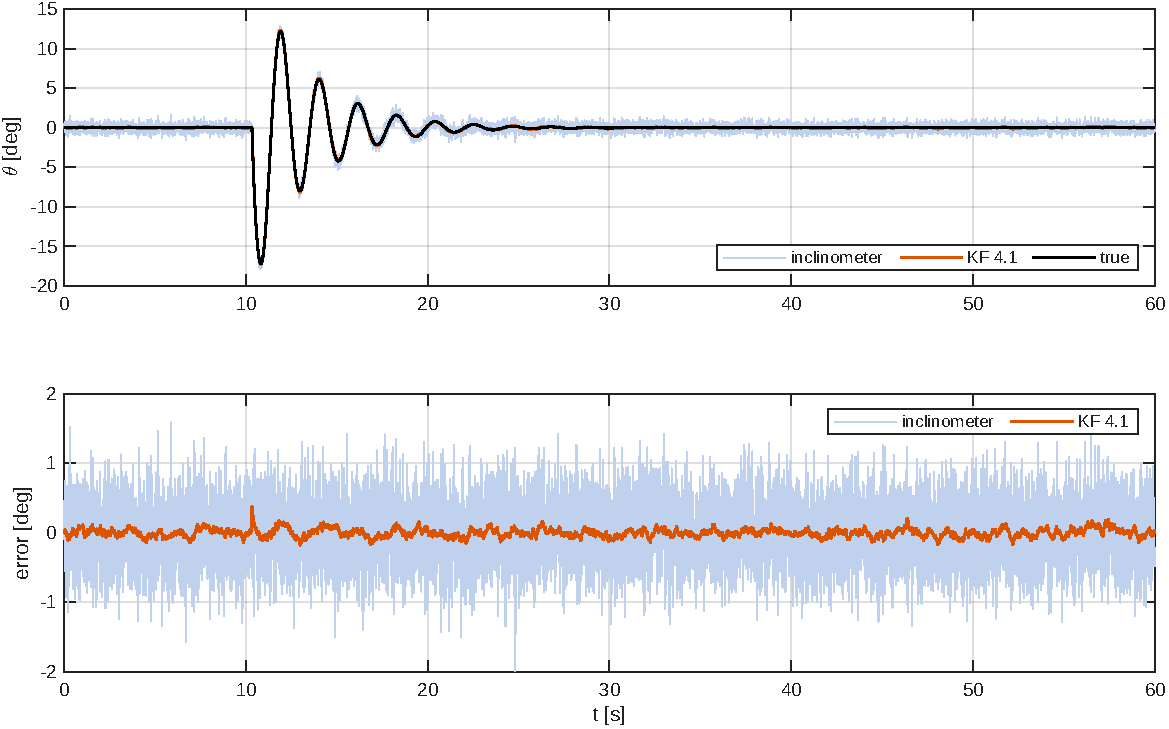
\includegraphics[width=0.7\linewidth]{figs/4_1_sim.pdf}
\captionof{figure}{Simulation without gyro bias, pitch: inclinometer, filter of Q4.1 and true angle (top) and estimation error (bottom).}
\label{fig:sim}
\end{center}
\end{answer}

% ------------------------------------------------------------ Q4.2 ---
\begin{question}{4.2}{T}
For constant Kalman gains obtain the transfer function from pitch inclinometer measurement $\theta_m$ to pitch estimate $\hat{\theta}$ and the transfer function from the rate-gyro measurement $\omega_{ym}$ to pitch estimate $\hat{\theta}$. Comment on the results
\end{question}

\begin{answer}

With constant gain $L_\theta$, the steady-state filter of Q4.1 is a linear time-invariant system. Taking Laplace transforms with zero initial conditions,
\[
  \dot{\hat\theta} = \omega_{y_m} + L_\theta\,(\theta_m-\hat\theta)
  \quad\Longrightarrow\quad
  s\hat\theta(s) = \omega_{y_m}(s) + L_\theta\,\big(\theta_m(s)-\hat\theta(s)\big),
\]
so
\begin{equation}
  \small
  \hat\theta(s) = \frac{L_\theta}{s+L_\theta}\,\theta_m(s) + \frac{1}{s+L_\theta}\,\omega_{y_m}(s)
  \,\Rightarrow\,
  \hat\theta(s) = \underbrace{\frac{L_\theta}{s+L_\theta}}_{G_L(s)}\,\theta_m(s)
  + \frac{1}{s}\,\underbrace{\frac{s}{s+L_\theta}}_{G_H(s)}\,\omega_{y_m}(s)
  \label{eq:q42_tf}
\end{equation}

The roll filter is identical, with $\phi_m$ (roll inclinometer), $\omega_{x_m}$ (roll rate gyro) and its own gain $L_\phi$ (computed from the roll $Q$ and $R$):
\begin{equation}
  \hat\phi(s) = \underbrace{\frac{L_\phi}{s+L_\phi}}_{G_L(s)}\,\phi_m(s)
  + \frac{1}{s}\,\underbrace{\frac{s}{s+L_\phi}}_{G_H(s)}\,\omega_{x_m}(s)
  \label{eq:q42_tf_roll}
\end{equation}
Hence the same block diagram applies to both axes (Fig.~\ref{fig:complementary-filter}).

\begin{center}
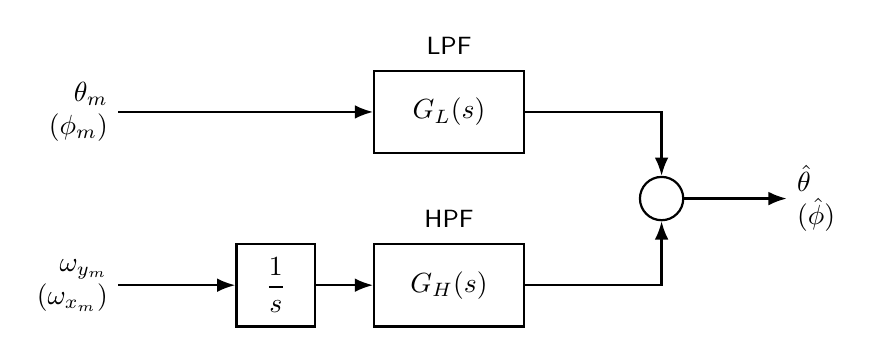
\begin{tikzpicture}[
    >=Latex,
    blk/.style={draw, thick, minimum width=1.9cm, minimum height=1.05cm, align=center},
    sblk/.style={draw, thick, minimum width=1.0cm, minimum height=1.05cm, align=center},
    lbl/.style={font=\small\sffamily, above=2pt},
    sig/.style={->, thick}
  ]
  \node[blk]  (GL)  at (4.2, 1.1)  {$G_L(s)$};
  \node[sblk] (INT) at (2.0,-1.1)  {$\dfrac{1}{s}$};
  \node[blk]  (GH)  at (4.2,-1.1)  {$G_H(s)$};
  \node[draw, thick, circle, minimum size=0.55cm, inner sep=0pt] (sum) at (6.9, 0) {};
  \node[lbl] at (GL.north) {LPF};
  \node[lbl] at (GH.north) {HPF};
  \draw[sig] (0,1.1)  node[left,align=right] {$\theta_m$\\$(\phi_m)$} -- (GL.west);
  \draw[sig] (0,-1.1) node[left,align=right] {$\omega_{y_m}$\\$(\omega_{x_m})$} -- (INT.west);
  \draw[sig] (INT.east) -- (GH.west);
  \draw[sig] (GL.east) -| (sum.north);
  \draw[sig] (GH.east) -| (sum.south);
  \draw[sig] (sum.east) -- ++(1.3,0) node[right,align=left] {$\hat\theta$\\$(\hat\phi)$};
\end{tikzpicture}
\captionof{figure}{Block diagram of the transfer function for pitch estimation; for roll, replace the signals by the ones in parentheses and $L_\theta$ by $L_\phi$.}
\label{fig:complementary-filter}
\end{center}

$G_L$ is a first-order low-pass filter with unit DC gain and $G_H$ a
first-order high-pass filter, both with cutoff frequency $L$. The
estimate uses the inclinometer at low frequency, where it does not
drift, and the integrated rate gyro at high frequency, where the
inclinometer is noisy. With $L_\theta = 3.62$\,rad/s the crossover is at
$0.58$\,Hz. A constant gyro bias $b_y$ is not rejected, since
$\tfrac{1}{s}G_H(0) = 1/L_\theta$: it gives a constant error
$b_y/L_\theta$ in the estimate.
\end{answer}

% ------------------------------------------------------------ Q4.3 ---
\begin{question}{4.3}{T}
Discuss the impact of changing the tuning parameters Q and R.
\end{question}

\begin{answer}

For the steady state Kalman Filter of Q4.1 the gain is
$L=\sqrt{R/Q}$, so only the ratio $R/Q$ matters, and $L$ is the cutoff
frequency of the two filters of Q4.2:
\begin{itemize}
  \item increasing $Q$ (or decreasing $R$) means trusting the
  inclinometer less: $L$ decreases, the estimate follows the integrated
  gyro for longer ($1/L$) and is less affected by vibration and by
  linear accelerations, but an initial error takes longer to correct
  and the error due to a gyro bias, $b/L$, increases;
  \item decreasing $Q$ (or increasing $R$) means trusting the
  inclinometer more: $L$ increases and the estimate tends to the raw
  inclinometer angle.
\end{itemize}

Fig.~\ref{fig:tuning} shows the filter of Q4.1 with $Q$, $10^2Q$ and
$10^4Q$. With the measured covariances ($L\approx 3.6$\,rad/s) the
estimate stays close to the inclinometer, which during the manoeuvres
does not follow the onboard angle. With $10^2 Q$ ($L\approx
0.36$\,rad/s) the estimate follows the onboard angle in the step. With
$10^4 Q$ the filter is almost a pure integration of the gyro and the
errors accumulated take $1/L\approx 28$\,s to be corrected.

\begin{center}
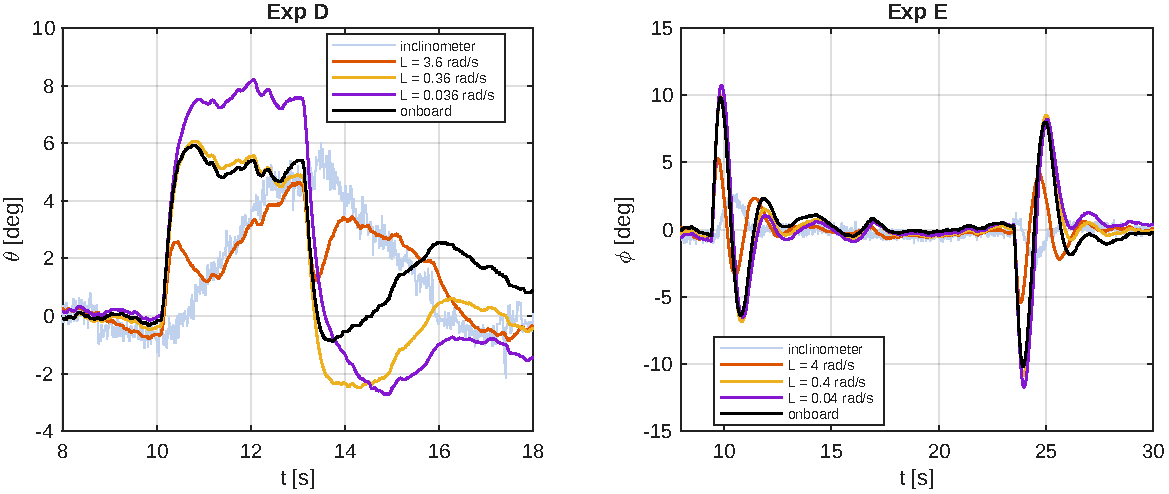
\includegraphics[width=0.85\linewidth]{figs/4_3_tuning.pdf}
\captionof{figure}{Filter of Q4.1 for three values of $Q$: pitch in Experiment D and roll in Experiment E.}
\label{fig:tuning}
\end{center}
\end{answer}

% ------------------------------------------------------------ Q4.4 ---
\begin{question}{4.4}{T+L}
Repeat the Kalman filter design, implementation, and evaluation procedure augmenting
the system with an extra state to capture the bias term on the rate gyro. For that purpose, assume
that
\[ \dot b_y = 0 \]
and
\[ w_{y_m} = q + b_y \]

Suggestion: In the simulation phase, set an artificial bias on the measurement and plot the bias $b_y$ vs. bias estimate $\hat{b}_y$ to guide the tuning of the filter.
\end{question}

\begin{answer}
With $q = \omega_{y_m} - b_y$ the model becomes
\[
  \dot\theta = \omega_{y_m} - b_y + w_\theta, \qquad
  \dot b_y = w_b, \qquad
  y_\theta = \theta + v_\theta ,
\]
where $w_b$ is a fictitious process noise of variance $R_b$ (with
$R_b=0$ the steady-state gain of the bias is zero). In state space,
with $x = [\theta \quad b_y]^T$ and $u=\omega_{y_m}$,
\[
  A = \begin{bmatrix} 0 & -1\\ 0 & 0 \end{bmatrix},\quad
  B = \begin{bmatrix} 1\\ 0 \end{bmatrix},\quad
  C = \begin{bmatrix} 1 & 0 \end{bmatrix},\qquad
  \mathrm{rank}\begin{bmatrix} C\\ CA \end{bmatrix}
  = \mathrm{rank}\begin{bmatrix} 1 & 0\\ 0 & -1 \end{bmatrix} = 2,
\]
so the bias is observable. The filter is
\[
\begin{aligned}
  &\dot{\hat\theta} = \omega_{y_m} - \hat b_y + L_1(\theta_m - \hat\theta)\\
  &\dot{\hat b}_y = L_2(\theta_m - \hat\theta)
\end{aligned}
\]
with $L = PC^TQ^{-1} = [p_{11} \quad p_{12}]^T/Q$. With
$P = \begin{bmatrix} p_{11} & p_{12}\\ p_{12} & p_{22}\end{bmatrix}$,
process noise $\mathrm{diag}(R,\,R_b)$ and measurement noise $Q$, the
three entries of $0 = AP + PA^T + \mathrm{diag}(R,R_b) - PC^TQ^{-1}CP$
are
\[
  (1,1):\ -2p_{12} + R - \frac{p_{11}^2}{Q} = 0, \qquad
  (1,2):\ -p_{22} - \frac{p_{11}p_{12}}{Q} = 0, \qquad
  (2,2):\ R_b - \frac{p_{12}^2}{Q} = 0 .
\]
From $(2,2)$, $p_{12} = -\sqrt{R_bQ}$ (the negative root gives a stable
filter), and then from $(1,1)$, $p_{11} = \sqrt{Q(R + 2\sqrt{R_bQ})}$, so
\[
  L_2 = \frac{p_{12}}{Q} = -\sqrt{R_b/Q}, \qquad
  L_1 = \frac{p_{11}}{Q} = \sqrt{R/Q + 2\sqrt{R_b/Q}} .
\]
The implementation is the same block of Q4.1 with the state
$[\phi \quad \theta \quad b_x \quad b_y]^T$.

\paragraph{Simulation}
In \texttt{ARDroneHoverSim\_4\_4} a constant bias $b_y = 0.05$\,rad/s
($2.86$\,deg/s) is added to the simulated gyro, with the same manoeuvre
and noise of Q4.1. Fig.~\ref{fig:sim-bias} (bottom) shows $\hat b_y$ for three
values of $R_b$. The poles are the roots of $s^2+L_1s-L_2$; the slow
one is approximately $L_2/L_1 \approx -\sqrt{R_b/R}$, so the bias
converges with a time constant of about $32$, $10$ and $3$\,s for
$R_b = 10^{-3}R$, $10^{-2}R$ and $10^{-1}R$. We chose $R_b=10^{-2}R$; for
pitch $\sqrt{R_b/Q} = \sqrt{0.131} = 0.362$ and
$L_1 = \sqrt{13.1 + 0.72} = 3.72$, and for both axes
\[
  L = \begin{bmatrix} 4.06 & 0\\ 0 & 3.72\\ -0.396 & 0\\ 0 & -0.362 \end{bmatrix}.
\]
With the bias, the filter of Q4.1 keeps a constant error of
$0.79^\circ$ $(= b_y/L_\theta)$, while the error of the augmented
filter goes to zero as the bias converges (RMS of $0.07^\circ$ for
$t\geq 20$\,s), Fig.~\ref{fig:sim-bias} (top).

\begin{center}
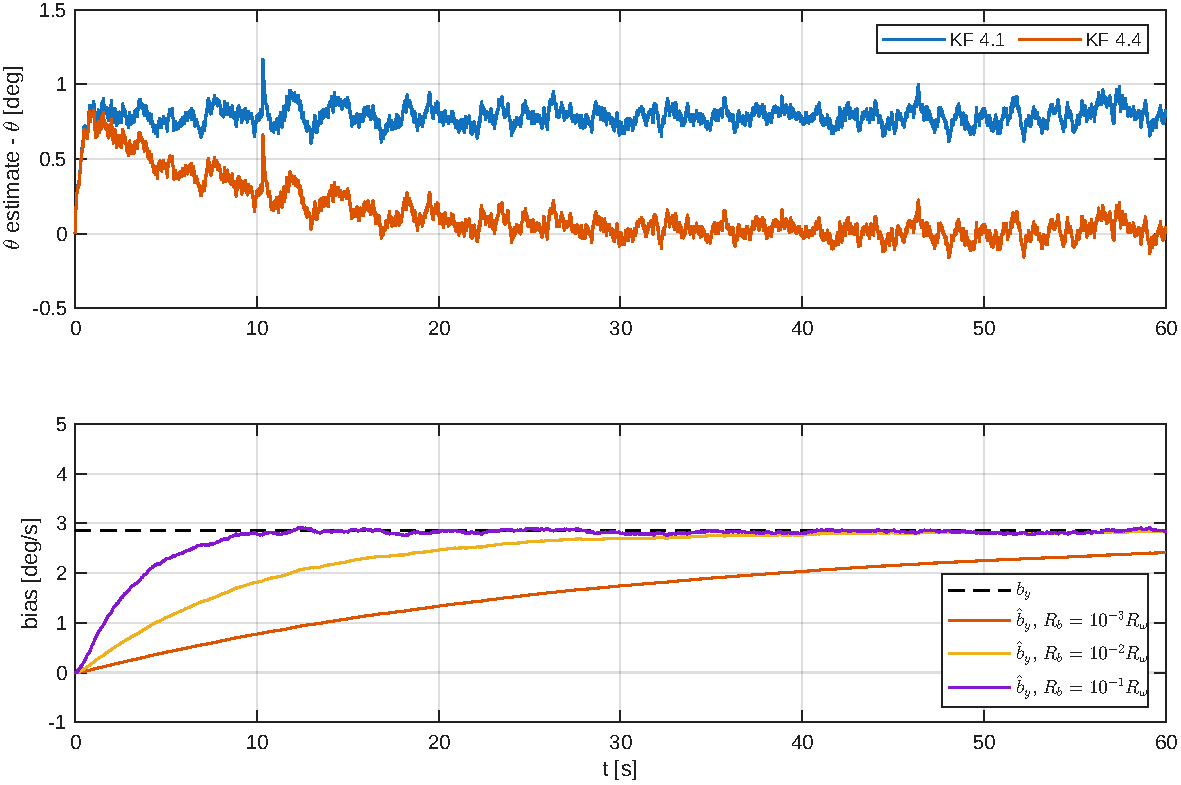
\includegraphics[width=0.7\linewidth]{figs/4_4_sim.pdf}
\captionof{figure}{Simulation with gyro bias $b_y = 0.05$\,rad/s: pitch error of the filters of Q4.1 and Q4.4 with $R_b=10^{-2}R$ (top); bias $b_y$ and its estimate $\hat b_y$ for three values of $R_b$ (bottom).}
\label{fig:sim-bias}
\end{center}

\paragraph{Experiments}
In the experimental data the bias estimated at rest (Experiment A) is
about $-0.1$\,deg/s in $y$ (the gyro mean of Q3.1 is $-0.085$\,deg/s)
and below $0.03$\,deg/s in $x$. With such a small bias the angles of the
two filters almost coincide (Figs.~\ref{fig:exp-pitch}
and~\ref{fig:exp-roll}).
\end{answer}

% ------------------------------------------------------------ Q4.5 ---
\begin{question}{4.5}{T}
Check if the previous filters are complementary. Discuss the advantages and limitations of
this class of filters.
\end{question}

\begin{answer}
Two filters are complementary if their transfer functions add up to one.
For the filter of Q4.1, from Eq.~\eqref{eq:q42_tf},
\[
  G_L(s) + G_H(s) = \frac{L_\theta}{s+L_\theta} + \frac{s}{s+L_\theta} = 1 .
\]
For the filter of Q4.4, the second equation gives
$\hat b_y = \tfrac{L_2}{s}(\theta_m - \hat\theta)$; replacing it in the
first one, $(s^2 + L_1 s - L_2)\,\hat\theta = s\,\omega_{y_m} + (L_1 s - L_2)\,\theta_m$, so
\[
  \hat\theta(s) = \underbrace{\frac{L_1 s - L_2}{s^2+L_1 s-L_2}}_{G_L(s)}\,\theta_m(s)
  + \frac{1}{s}\,\underbrace{\frac{s^2}{s^2+L_1 s-L_2}}_{G_H(s)}\,\omega_{y_m}(s),
  \qquad G_L(s)+G_H(s) = 1 .
\]
Both are complementary (Fig.~\ref{fig:bode}). In the second one $G_H$ is
of second order, so $\tfrac{1}{s}G_H(0)=0$ and a constant gyro bias is
rejected.

\begin{center}
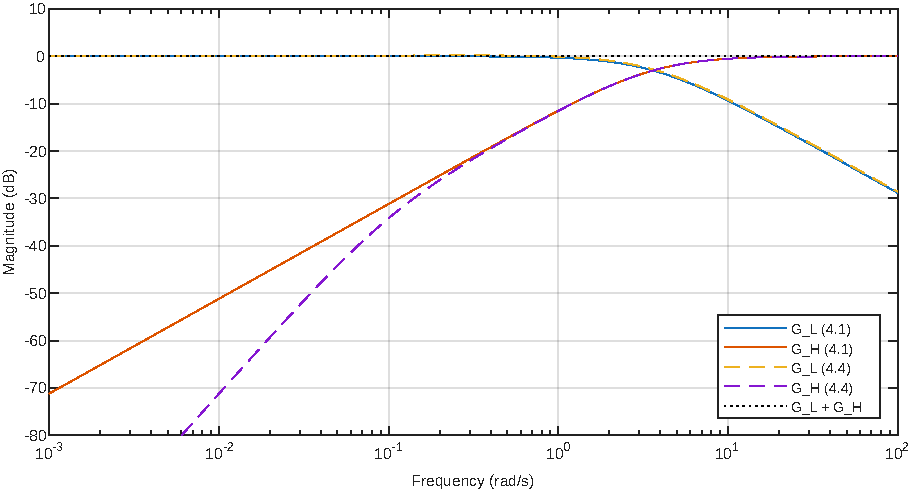
\includegraphics[width=0.7\linewidth]{figs/4_5_bode.pdf}
\captionof{figure}{Magnitude of the complementary filters of Q4.1 and Q4.4 (pitch).}
\label{fig:bode}
\end{center}

Advantages: if both sensors measure the same angle, $\theta_m=\theta$
and $\omega_{y_m}=s\theta$, then $\hat\theta=\theta$ at all frequencies,
so the filter introduces no lag or attenuation on the signal and only
filters the noise; no model of the vehicle dynamics is needed; the
implementation is one integrator and one gain per axis.

Limitations: the errors of the two sensors have to be separated in
frequency. The low-frequency errors of the inclinometer (accelerometer
offset, linear accelerations) and the high-frequency noise of the gyro
pass to the estimate. The gains are constant, so the trade-off chosen
for one condition (hover) is kept in all the others.
\end{answer}

% ------------------------------------------------------------ Q4.6 ---
\begin{question}{4.6}{L}
Discuss the results obtained and relate them to the different conditions of operation specified in experiments A to E.
\end{question}

\begin{answer}
Figs.~\ref{fig:exp-pitch} and~\ref{fig:exp-roll} show the two filters,
the raw inclinometer and the onboard estimate. The onboard estimate is
the output of the drone's own filter, which uses the same sensors, so it
is not the true attitude (only known in simulation) and the differences
below are not errors of our filters. It is used for comparison because,
during the manoeuvres, its time derivative agrees with the rate gyro
(correlation coefficient of $0.94$ in D and $0.98$ in E).

\begin{center}
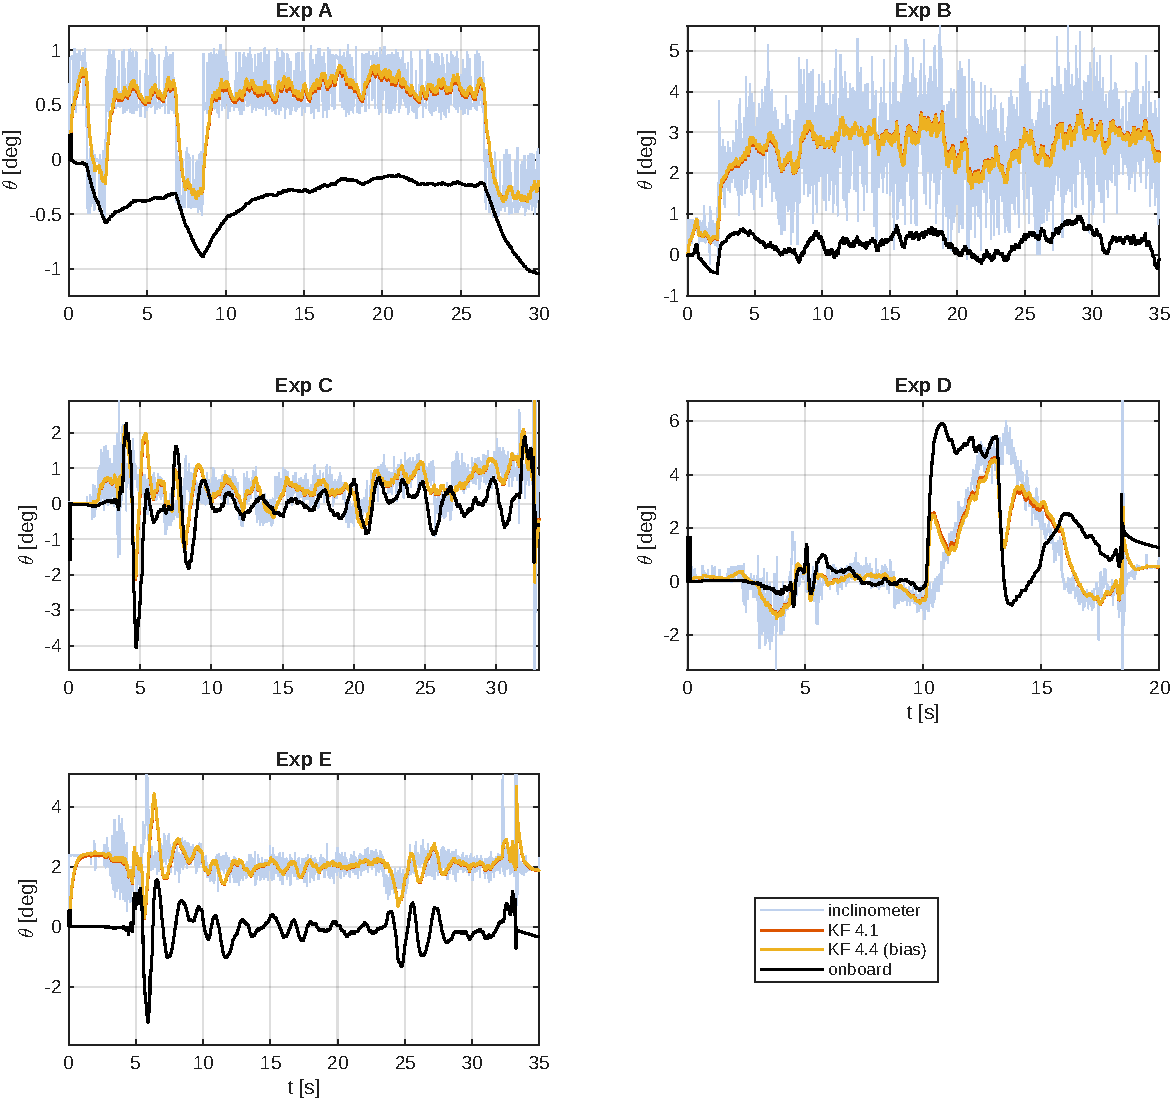
\includegraphics[width=0.78\linewidth]{figs/4_6_pitch.pdf}
\captionof{figure}{Pitch in Experiments A to E.}
\label{fig:exp-pitch}
\end{center}

\begin{center}
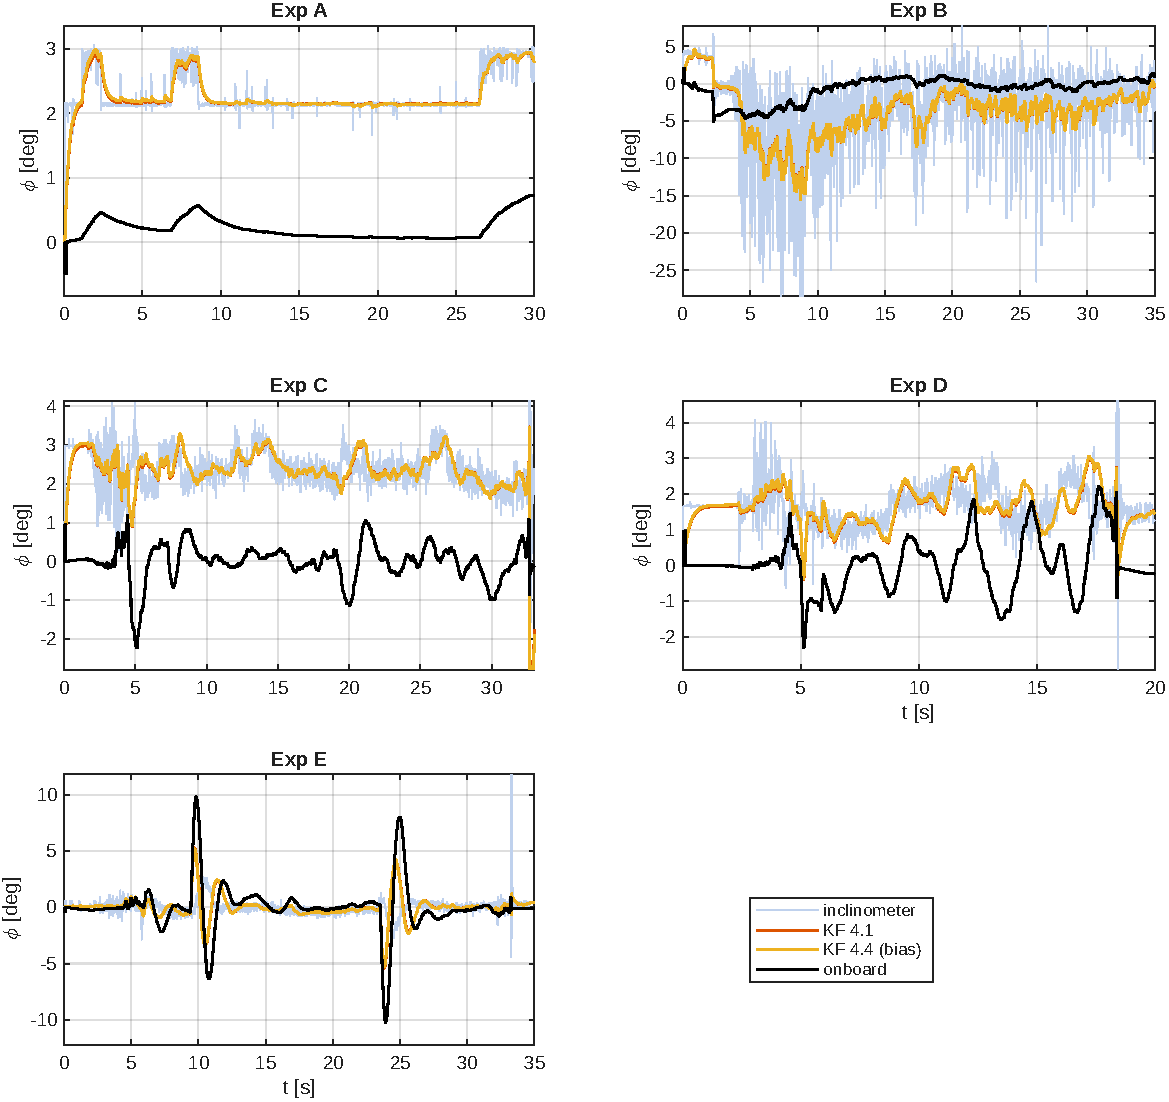
\includegraphics[width=0.78\linewidth]{figs/4_6_roll.pdf}
\captionof{figure}{Roll in Experiments A to E.}
\label{fig:exp-roll}
\end{center}

\begin{itemize}
  \item \textbf{A (at rest):} the estimate is the inclinometer without
  the noise (standard deviation from $0.19^\circ$ to $0.07^\circ$ in
  pitch). There is a constant difference to the onboard estimate
  ($0.9^\circ$ in pitch, $2.0^\circ$ in roll), which is the offset of
  the raw inclinometer seen in Q3.4. Our filters use the inclinometer as
  the only absolute measurement and keep it; the onboard filter probably
  removes it with its own calibration.
  \item \textbf{B (rotors on, on the ground):} the vibration increases
  the inclinometer noise and also moves its mean (roll of $-3.5^\circ$
  with the drone on the ground). The filter removes the high-frequency
  part (standard deviation of the roll from $4.5^\circ$ to
  $1.8^\circ$) but follows the low-frequency part, so this is the
  experiment with the largest difference to the onboard estimate.
  \item \textbf{C (hover):} the estimate follows the mean of the
  inclinometer. Its standard deviation is only slightly lower
  ($0.44^\circ$ to $0.38^\circ$ in pitch), so most of the variance
  measured in hover is at low frequency, below $L$, and is not removed.
  \item \textbf{D (pitch step):} the onboard pitch goes to about
  $5.4^\circ$ in the first second of the step, while the inclinometer
  takes about $3$\,s to get there. In flight the accelerometer measures
  the specific force and not only gravity, so the inclinometer does not
  give the tilt during the acceleration. The filter follows the gyro
  only for $1/L_\theta\approx 0.3$\,s and then goes to the
  inclinometer: its mean in the first second is $1.8^\circ$.
  \item \textbf{E (waypoints in $y$):} the same happens in roll, where
  the onboard estimate has peaks of $9.8^\circ$ and $-6.4^\circ$, and
  the filter only $5.3^\circ$ and $-3.3^\circ$.
\end{itemize}

The $Q$ and $R$ measured in hover describe the noise of the sensors but
not the error of the inclinometer during manoeuvres. For D and E a
lower gain, which relies more on the gyro, gives an estimate closer to
the onboard one (Fig.~\ref{fig:tuning}).

The filter with bias gives almost the same angles in all experiments.
Its bias estimate stays within $\pm0.2$\,deg/s in A and C, but reaches
$\pm0.6$\,deg/s in $\hat b_y$ during the step of D, $\pm0.8$\,deg/s in
$\hat b_x$ during the manoeuvres of E, and $-0.6$\,deg/s in $\hat b_x$
in B: the difference between the gyro and the inclinometer in these
conditions is taken as bias.
\end{answer}

% ------------------------------------------------------------ Q4.7 ---
\begin{question}{4.7}{T+L}
Repeat the previous questions for the roll estimation.
\end{question}

\begin{answer}
No separate derivation is needed for roll, since the pitch and roll
channels are decoupled and share the same structure. Every design, transfer
function and result of Questions 4.1--4.6 was therefore obtained for
both angles, using the following correspondence:
\[
  \theta \to \phi, \qquad
  \omega_{y_m} \to \omega_{x_m}, \qquad
  \theta_m \to \phi_m, \qquad
  b_y \to b_x .
\]
The steady-state gains $L$ for roll (Q4.1), the bias-augmented
filter (Q4.4) and the evaluation on Experiments A to E (Q4.6) are
reported together with the pitch results, in the same tables and figures.
The conclusions on the complementarity of the filters (Q4.5) and on the
effect of $Q$ and $R$ (Q4.3) hold unchanged for roll.
\end{answer}

% =====================================================================
\section{Integrated roll and pitch estimation}

% -------------------------------------------------------------- Q5 ---
\begin{question}{5}{L}
Study and implement the solution proposed in P.~Batista, C.~Silvestre, and P.~Oliveira, ``Partial Attitude and Rate Gyro Bias Estimation: Observability Analysis, Filter Design, and Performance Evaluation,'' International Journal of Control, vol.~84, no.~5, pp.~895--903, May 2011. Note that you are only required to implement a Kalman filter for the nominal system (2) of the above-mentioned reference to partially estimate the attitude of the vehicle together with the bias of the three rate gyro components.
\end{question}

\begin{answer}
\paragraph{Nominal system}
Let $R$ be the rotation matrix from $\fB$ to $\fI$, with
$\dot R = R\,S(\omega)$, where $S(\cdot)$ is the skew-symmetric matrix
of the cross product. The direction of gravity in $\fB$,
$x = R^Te_3$, is constant in $\fI$, so $\dot x = -S(\omega)x$. The rate
gyro measures $\omega_m = \omega + b$ with constant bias $b$, and the
accelerometer measures $-x$ (in g) when the linear acceleration is
small. The nominal system is
\[
  \dot x = -S(\omega_m)\,x + S(b)\,x, \qquad \dot b = 0, \qquad y = x .
\]
It is nonlinear because of $S(b)x$, but since $S(b)x = -S(x)b$ and
$x=y$ is measured, it can be written as
\[
  \begin{bmatrix}\dot x\\ \dot b\end{bmatrix} =
  \underbrace{\begin{bmatrix} -S(\omega_m(t)) & -S(y(t))\\ 0 & 0 \end{bmatrix}}_{A(t)}
  \begin{bmatrix} x\\ b\end{bmatrix},
  \qquad
  y = \underbrace{\begin{bmatrix} I_3 & 0 \end{bmatrix}}_{C}
  \begin{bmatrix} x\\ b\end{bmatrix},
\]
which is system (2) of the reference, with $x_1 = x$ and $x_2 = b$. It
is treated as linear time-varying, since $\omega_m(t)$ and $y(t)$ are
known signals. There is no linearization and no small-angle
approximation.
Roll and pitch follow from
$x = [-\sin\theta \quad \sin\phi\cos\theta \quad \cos\phi\cos\theta]^T$,
\[
  \hat\phi = \operatorname{atan2}(\hat x_2,\,\hat x_3), \qquad
  \hat\theta = \operatorname{atan2}\!\big(-\hat x_1,\,\sqrt{\hat x_2^2+\hat x_3^2}\big),
\]
the inclinometer of Q3.4 applied to the filtered vector. The yaw angle
is not estimated (partial attitude).

\paragraph{Kalman filter}
The gyro noise $w_\omega$ enters as $\omega_m = \omega + b + w_\omega$,
so in $\dot x$ it appears as $-S(y)\,w_\omega$; as in Q4.4, a noise
$w_b$ is added to $\dot b$. With $G(t) = \mathrm{diag}(-S(y),\, I_3)$,
process noise $R = \mathrm{diag}(R_\omega,\, R_b)$ and measurement noise
$Q$ (accelerometer), the filter is
\[
\begin{aligned}
  &\dot{\hat{\mathbf{x}}} = A(t)\,\hat{\mathbf{x}} + L(t)\,(y - C\hat{\mathbf{x}}),
  \qquad L(t) = P(t)\,C^TQ^{-1},\\
  &\dot P = A(t)P + PA^T(t) + G(t)\,R\,G^T(t) - PC^TQ^{-1}CP, \qquad P(0)=P_0 ,
\end{aligned}
\]
with $\hat{\mathbf{x}} = [\hat x^T \quad \hat b^T]^T$. It is the
Riccati equation of Q4.1 without $\dot P = 0$: $A$ and $G$ change with
the measurements, so the gain is not constant and $P$ is integrated
together with the state. In the notation of the reference (Section 4),
$\Xi(t) = G(t)RG^T(t)$, $\Theta = Q$ and the gain is $K(t)$.

\paragraph{Observability}
$x$ is measured, so the question is the bias. It acts on $x$ through
$-S(y)b = b\times y$, which is zero for the component of $b$ parallel to
$y$. For constant $\omega_m$ and $y$,
\[
  \mathrm{rank}\begin{bmatrix} C\\ CA \end{bmatrix}
  = \mathrm{rank}\begin{bmatrix} I_3 & 0\\ -S(\omega_m) & -S(y) \end{bmatrix}
  = 3 + \mathrm{rank}\,S(y) = 5 ,
\]
and the higher powers of $A$ add nothing. In the reference, the system
is observable on $[t_0,t_f]$ if and only if $y$ is not constant in that
interval (Theorem 3.3), and uniformly completely observable, which makes
the Kalman filter error globally asymptotically stable, if the direction
of $y$ in $\fB$ keeps changing (Theorem 3.4). In hover $y\approx e_3$, so $b_x$ and $b_y$ are
observable and $b_z$ is not; a rotation in yaw does not change $y$ and
does not help. $b_z$ is only corrected while the vehicle is tilted.

\paragraph{Implementation}
The filter is one MATLAB Function block that computes
$\dot{\hat{\mathbf{x}}}$ and $\dot P$, followed by two integrators with
initial conditions $\hat{\mathbf{x}}_0$ and $P_0$. The inputs are the
rate gyro in rad/s and $y = -a/1000$, with $a$ the accelerometer in mg.
$R_\omega$ and $Q$ are the variances measured in hover (Q3.3),
\[
  R_\omega = \mathrm{diag}(6.38,\ 7.63,\ 7.77)\times10^{-4}\ (\mathrm{rad/s})^2, \qquad
  Q = \mathrm{diag}(5.91,\ 4.31,\ 5.68)\times10^{-5}\ \mathrm{g}^2,
\]
with $R_b = 10^{-4}R_\omega$,
$\hat{\mathbf{x}}_0 = [0 \quad 0 \quad 1 \quad 0 \quad 0 \quad 0]^T$
(level, no bias; the reference uses the first measurement, but the
first samples of the logs are zero) and
$P_0 = \mathrm{diag}(10^{-3}I_3,\ 0.05^2 I_3)$.
Here $P_0$ already gives a gain to the bias, so $R_b$ can be much
smaller than in Q4.4, where the steady-state bias gain was zero for
$R_b=0$.

\paragraph{Simulation}
In \texttt{ARDroneHoverSim\_5} the gyro is computed from the Euler angles
of the simulator and their derivatives,
$\omega = W(\phi,\theta)\,[\dot\phi \quad \dot\theta \quad \dot\psi]^T$,
plus noise of variance $R_\omega$ and a bias
$b = [-1.72 \quad 2.86 \quad 2.29]^T$\,deg/s; the accelerometer is
$x(\phi,\theta)$ plus noise of variance $Q$. Steps of 1\,m in $x$
($t=10$\,s) and $y$ ($t=30$\,s) give pitch up to $17^\circ$ and roll up
to $9^\circ$ (Fig.~\ref{fig:sim5}). $\hat b_x$ and $\hat b_y$ converge in
about 5\,s; $\hat b_z$ stays at zero, with its initial standard deviation
of $2.86$\,deg/s, until the step at 10\,s, and then moves only to
$0.57$\,deg/s, with $\sigma_{b_z}=2.5$\,deg/s. The RMS error of the angles
for $t\geq20$\,s is $0.06^\circ$, against $0.4^\circ$ for the
inclinometer.

\begin{center}
\begin{minipage}{\linewidth}\centering
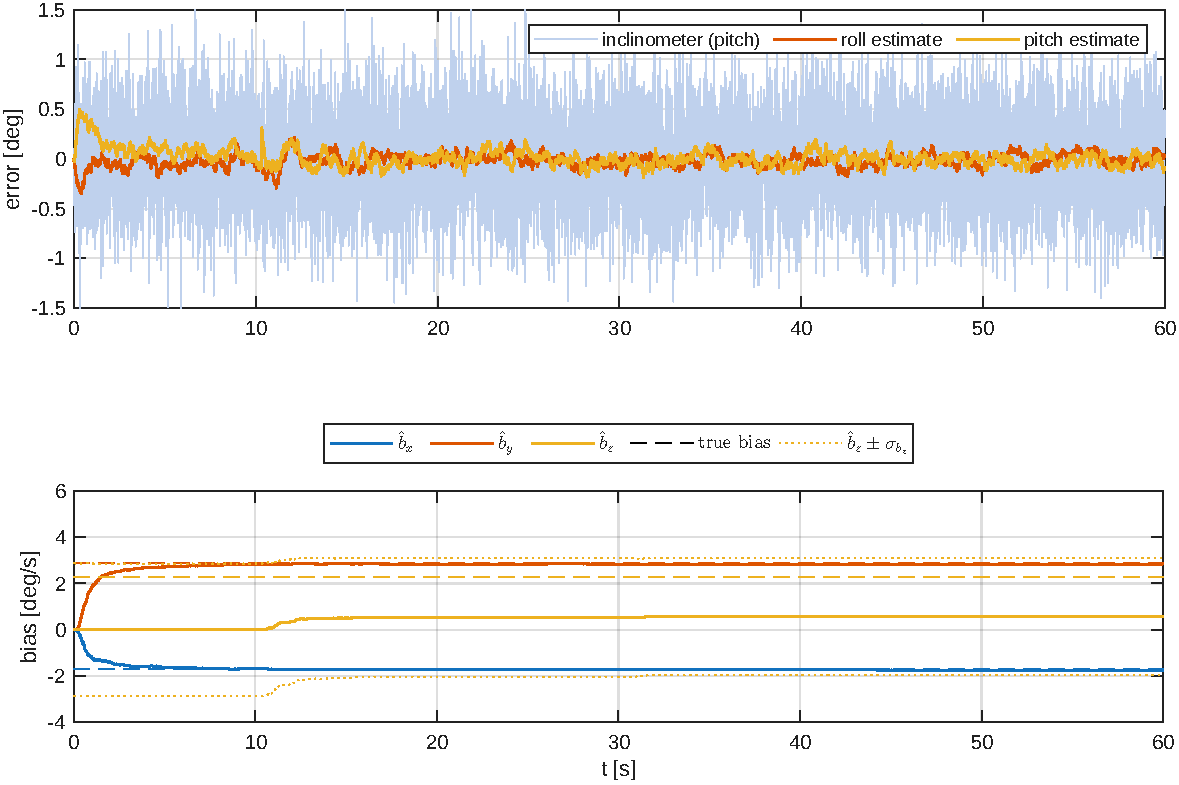
\includegraphics[width=0.68\linewidth]{figs/5_sim.pdf}
\captionof{figure}{Simulation with gyro bias in the three axes: angle error (top), bias and estimate (bottom).}
\label{fig:sim5}
\end{minipage}
\end{center}

\paragraph{Experiments}
Fig.~\ref{fig:exp5} compares the filter with the inclinometer, the
onboard estimate and the filter of Q4.4, with the measured $Q$ and with
$100\,Q$ (as in Q4.3). Table~\ref{tab:rms5} gives the RMS difference to
the onboard estimate, $\sqrt{\tfrac{1}{N}\sum_k(\hat\theta_k-\theta_{\mathrm{ob},k})^2}$,
in the intervals $10$--$24$, $10$--$33$, $9$--$30$, $6$--$18$ and
$8$--$32$\,s for A to E (those of Section 3 for A to C, and the flight
for D and E).

\begin{center}
\begin{minipage}{\linewidth}\centering
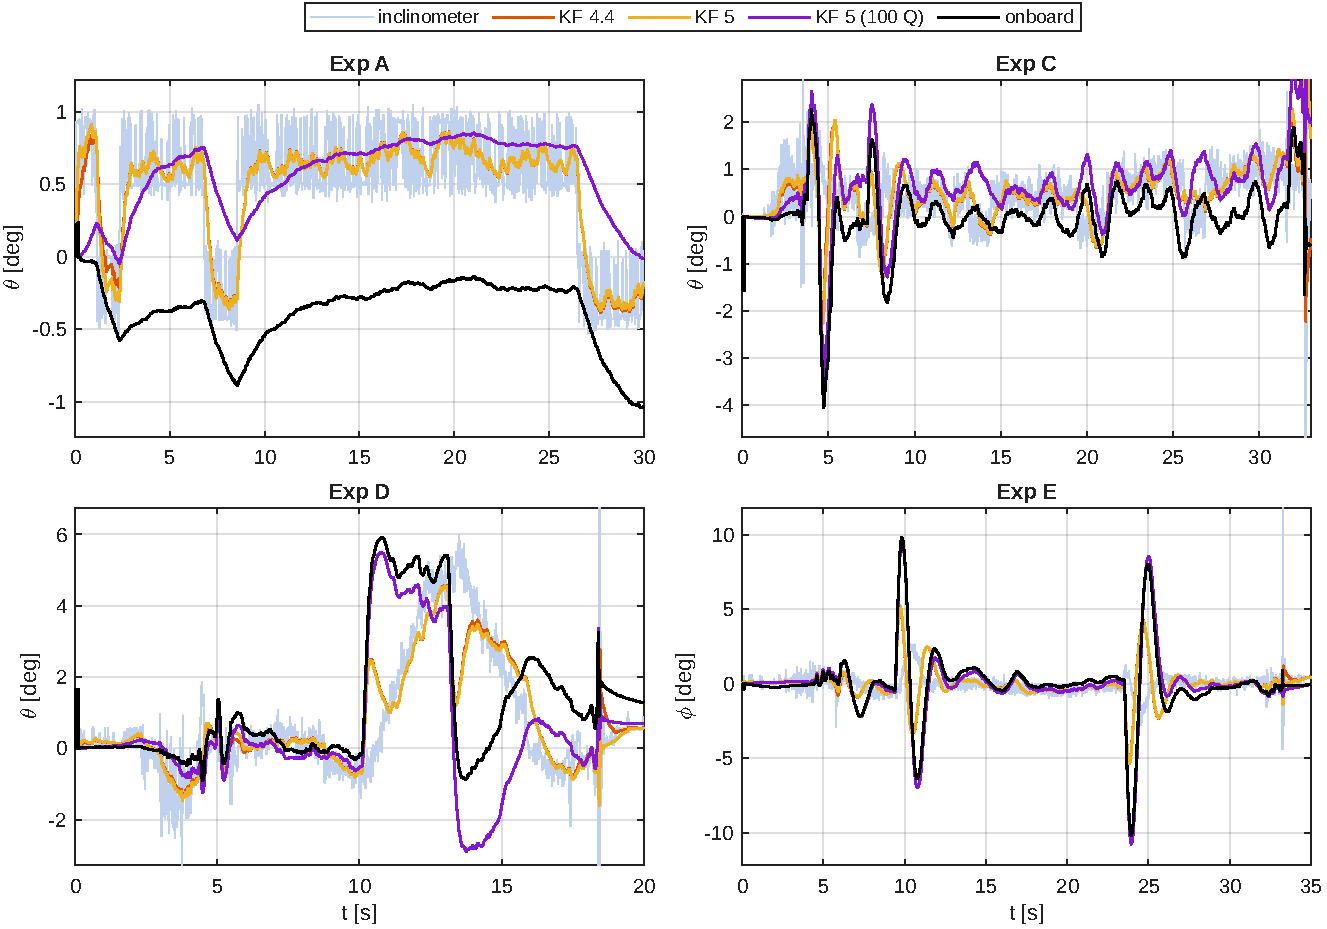
\includegraphics[width=0.8\linewidth]{figs/5_angles.pdf}
\captionof{figure}{Pitch in Experiments A, C and D and roll in Experiment E.}
\label{fig:exp5}
\end{minipage}
\end{center}

\begin{center}
\begin{minipage}{\linewidth}\centering
\small
\begin{tabular}{@{}l|rrrr|rrrr@{}}
\toprule
 & \multicolumn{4}{c|}{roll [deg]} & \multicolumn{4}{c}{pitch [deg]}\\
Exp. & incl. & KF 4.4 & KF 5 & KF 5 ($100Q$) & incl. & KF 4.4 & KF 5 & KF 5 ($100Q$)\\
\midrule
A & 2.02 & 2.03 & 2.03 & 2.29 & 0.96 & 0.95 & 0.95 & 0.99\\
B & 5.66 & 3.93 & 4.00 & 5.00 & 2.55 & 2.41 & 2.43 & 2.89\\
C & 2.46 & 2.42 & 2.42 & 2.66 & 0.65 & 0.54 & 0.55 & 0.67\\
D & 1.95 & 1.84 & 1.85 & 2.06 & 2.50 & 2.02 & 2.00 & 1.29\\
E & 2.72 & 1.92 & 1.91 & 0.46 & 2.16 & 2.15 & 2.15 & 2.35\\
\bottomrule
\end{tabular}
\captionof{table}{RMS difference to the onboard estimate.}
\label{tab:rms5}
\end{minipage}
\end{center}

With the measured $Q$ the angles are almost the same as those of Q4.4:
for small angles $x\approx[-\theta \quad \phi \quad 1]^T$ and
$-S(\omega_m)x\approx[-q \quad p \quad 0]^T$, so the first two components
reduce to the two filters of Q4.4. The constant roll offset of about
$2^\circ$ (A, C) is the inclinometer offset of Q3.4. With $100\,Q$ the
filter follows the onboard roll in E (RMS from $1.91^\circ$ to
$0.46^\circ$) and the start of the pitch step in D ($\hat\theta$ passes
$4^\circ$ at 10.4\,s, the onboard at 10.3\,s, the filter with $Q$ only at
12.7\,s). After the step, however, $\hat\theta$ is up to $2.6^\circ$
below the onboard value: with a lower gain the errors of the integrated
gyro take longer, $1/L$, to be corrected.

\begin{center}
\begin{minipage}{\linewidth}\centering
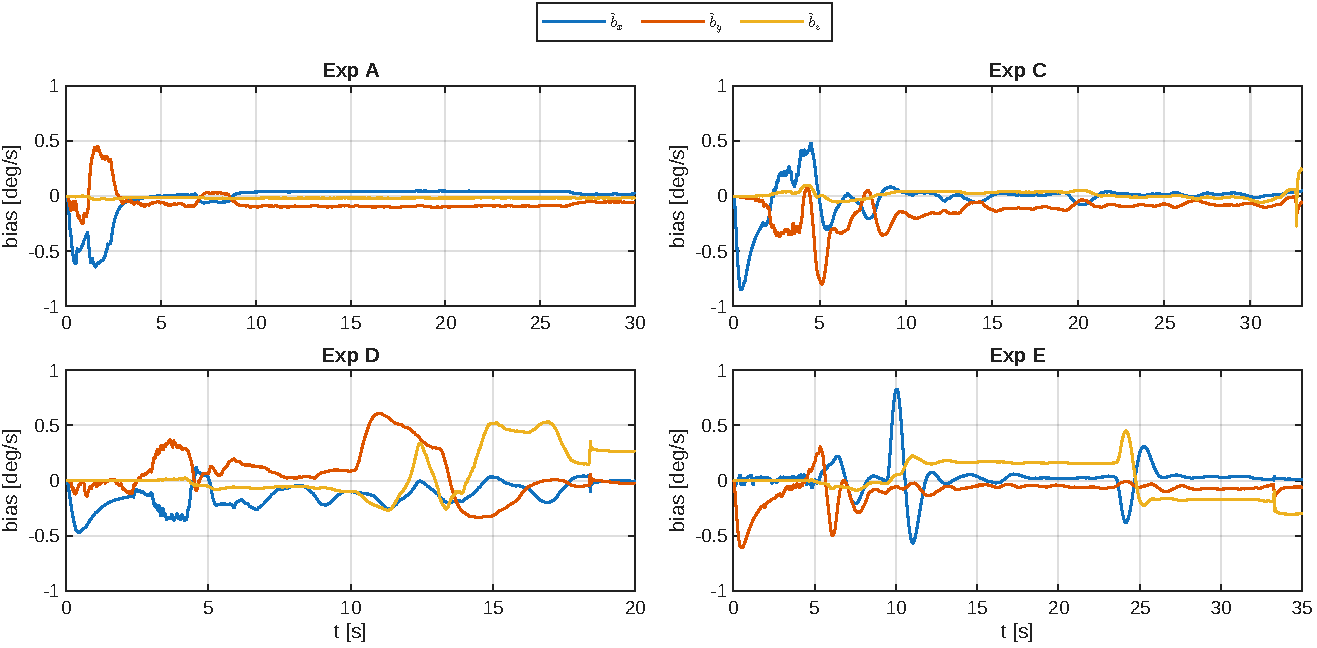
\includegraphics[width=0.72\linewidth]{figs/5_bias.pdf}
\captionof{figure}{Bias estimate of the three rate gyros (measured $Q$).}
\label{fig:bias5}
\end{minipage}
\end{center}

At rest (A) $\hat b$ converges in about 5\,s to
$[0.044 \quad -0.093 \quad -0.017]$\,deg/s, close to the mean of the
gyro in Q3.1, $[0.048 \quad -0.085 \quad 0.003]$\,deg/s
(Fig.~\ref{fig:bias5}). $\sigma_{b_x}$ and $\sigma_{b_y}$ fall to about
$0.3$\,deg/s in all the experiments, while $\sigma_{b_z}$ stays at
$2.8$\,deg/s, the initial value, in A, C, D and E: the vehicle is never
tilted enough for $b_z$ to be observable. $\hat b_z$ only moves during
the manoeuvres of D and E (up to $0.5$\,deg/s), and there the change
comes from the linear acceleration, which the model takes as a rotation
of $y$, and not from the bias. In the same manoeuvres $\hat b_x$ and
$\hat b_y$ reach $0.8$\,deg/s, as in Q4.4.
\end{answer}

\end{document}

